\documentclass[11pt]{article}
\pagestyle{empty}

\setlength{\textheight}{8.5in}
\setlength{\topmargin}{0.5in}
\setlength{\headheight}{0in}
\setlength{\headsep}{0in}
% %% \setlength{\footheight}{0in}
\setlength{\oddsidemargin}{0in}
\setlength{\textwidth}{6.5in}

\usepackage{times}
\usepackage{url}
\usepackage{algorithm}
\usepackage{mathtools}
\usepackage{mathptmx}
\usepackage{amssymb}
\usepackage{color}
\usepackage{graphicx}

\begin{document}
\sloppy 
\begin{center}
\LARGE CAS CS 132\\
\Large Geometric Algorithms\\
\Large\rm Spring 2020\\~\\
\end{center}

\noindent{\large\bf Meeting Place:} STO B50\\[\baselineskip]
\noindent{\large\bf Meeting
Time:} TR 3:30 pm -- 4:45 pm 
\\[\baselineskip] 

\noindent{\large\bf Instructor:} Prof.\ Mark Crovella\\[0.75\baselineskip]
\begin{minipage}[t]{0.60\textwidth}
\begin{itemize}
\item {\bf Office Hours:} See calendar below.
\item {\bf Office Hours Location:} MCS-101B 
\item {\bf Email:} \texttt{crovella@bu.edu}
\end{itemize}
\end{minipage}
~\\~\\~\\~\\
 \begin{minipage}[t]{0.60\textwidth}
 \noindent{\large\bf Teaching Fellow:} Nathan Cordner 
 \begin{itemize}
 \item {\bf Office Hours:} See calendar below.
% phone is 385-208-2370, office: MCS 117C
 \item {\bf Office Hours Location:} MCS B32
 \item {\bf Email:} \texttt{ncordner@bu.edu}
 \end{itemize}
 \end{minipage}
 \begin{minipage}[t]{0.60\textwidth}
 \noindent{\large\bf Teaching Fellow:} Max Heldman
 \begin{itemize}
 \item {\bf Office Hours:} See calendar below.
 \item {\bf Office Hours Location:} EMA 302.
 \item {\bf Email:} \texttt{heldmanm@bu.edu}
 \end{itemize}
 \end{minipage}
~\\~\\~\\
\textbf{Course Assistants (see calendar below for office hours):}  
\begin{itemize}
\item Drew Abram, \texttt{abramd@bu.edu}
\item Cali Dolfi, \texttt{cdolfi@bu.edu}
\item Myles Hayes, \texttt{mhayes18@bu.edu}
\item Bjoern Hasemann, \texttt{bjoernh@bu.edu}
\item Keshav Maheshwari, \texttt{km02@bu.edu}
\item Snigdha Kalathur, \texttt{srk22@bu.edu}
\end{itemize}

\newpage
\section*{Overview of the Course}

This course will introduce you to linear algebra from a Computer Science
standpoint.  Linear algebra is such a useful tool that it is crucially
important to a number of areas in Computer Science. For example, if you study
optimization, the starting point is linear algebra. If you study
computer graphics, the language you use every day is linear algebra. If
you study the performance of computer systems, you need linear
algebra. If you study algorithms -- especially graph algorithms -- you
will absolutely need linear algebra. If you study data mining, you will
use linear algebra all the time. 

The dominance of linear algebra arises because it is so fundamental, and
in some ways, very simple. It deals with objects that almost always can
be interpreted geometrically. So often we can use linear algebra in a
very intuitive manner -- so much so that many times it is actually the
best way to think about geometric problems. But it is also rigorous --
and so it
captures situations that sometimes we might overlook if we were
proceeding purely intuitively.  So the
advantage of being basic and fundamental is that it can be used and
applied in so many ways. 

As mentioned already, this course is taught from a computer science
perspective.  As such, it 
seeks to develop (simultaneously) three different modes of thinking:
algebraic, geometric, and computational.    To support this, the course
makes heavy use of interactive technology and you will be expected to do
significant programming.    There is more information about the teaching
philosophy of the course in the ``CS 132 Teaching Philosophy'' document
in the course repository.

\section*{Getting Set Up}

You will need to set up access to the following online materials.
Instructions for how to do all of those setups are below.   Note the
first five are \textbf{required;}  Using Github and DiagramAR are
\textbf{not}  required but \textbf{highly recommended.}

\begin{description}
\item[Required] The online textbook \emph{Linear Algebra and Its
  Applications} (LAA),
\item[Required] Python on your laptop for homeworks, 
\item[Required] Tophat for inclass participation,
\item[Required] Piazza for discussion of assignments and course material,
\item[Required] Gradescope for assignment submission, 
\item[Recommended] the course \texttt{Github} repository, for access to
  the lecture slide (and for experimenting with them), and
\item[Recommended] the visualization app \texttt{DiagramAR,} for
  studying and interacting with figures via augmented reality.
\end{description}

\section*{Textbook} 

The text for the course is \emph{Linear Algebra and
  Its Applications} (LAA), 5th edition, by David C. Lay, Steven R. Lay,
and Judi J. McDonald.    

Lectures are closely tied to book sections, and you will get
the most out of lecture if you read the corresponding book section
beforehand.   You will also want to refer to the book when you are doing
homeworks.   See the reading schedule at the end of the syllabus.

You do \textbf{not} need to buy a hardcopy of this textbook!
We will use an online textbook for this course, via a product called
\texttt{MyMathLab}.   This online text is 
being provided free of charge by the publisher, on a trial basis.   We
only ask that you provide short feedback in the form of a digital
survey at the end of the course.
\\
~\\\emph{\textbf{Setup}: Step-by-step instructions for accessing MyMathLab are on
  Piazza.  In brief: go to \url{https://www.pearson.com/mylab}, select
  Register as a Student.   The instructor's course ID is crovella29991.
Create an account if you don't have one, then select the access code
option, and enter the access code WSCMMV-PASHM-ILMEN-COMET-DOLBY-VEXES.
To view the text, you will also need to install the Wolfram CDF viewer on
your local machine (available from the Pearson site).}

\section*{Programming Environment}

We will use \texttt{python} as the language for teaching and for
assignments that require coding.    You are expected to know python and
to use it for all coding assignments.
\\
~\\\noindent\emph{\textbf{Setup}: Instructions for installing and
using Python are on Piazza.}

\section*{Tophat}

We will be using ``Peer instruction'' as part of the lectures.  This
requires you to answer questions during lecture, sometimes
after discussion with your classmates.   

To support this, we will use Tophat (\url{www.tophat.com}) for student
feedback during lecture. You will be able to submit answers to in-class
questions using Apple or Android smartphones and tablets, laptops, or
through text message. 

Should you require assistance with Top Hat at any time, due to the fact
that they require specific user information to troubleshoot these
issues, please contact their Support Team directly by way of email
(\texttt{support@tophat.com}), the in-app support button, or by calling
1-888-663-5491. 

You will also want to bring pencil and paper to lecture.   This isn't
absolutely critical, but you will find it easier if you can jot a note
or two while responding to in-class questions.
\\
~\\\emph{\textbf{Setup:} If you registered before the semester start,
  you should have gotten an email with instructions for how to create
  your account and sign in.  If you are adding the
  class late, you can register using the join code: 794726; if you have
  problems, please contact a TF.} 

\section*{Piazza}

We will be using Piazza for class discussion. The system is well
tuned to getting you help fast and efficiently from classmates, TFs,
CAs,
and myself. Rather than emailing questions to the teaching staff,
please post your questions on Piazza.  
We will also use Piazza for distributing materials
such as homeworks and helpful resources.

When someone posts a question on Piazza, if you know the answer, please
go ahead and post it.   However pleased \emph{don't} provide answers to homework
questions on Piazza.   It's OK to tell people \emph{where to look} to
get answers, or to correct mistakes;  just don't provide actual solutions
to homeworks.
\\
~\\\emph{\textbf{Setup:}  Our class Piazza
page  is at \url{piazza.com/bu/spring2020/cs132/home}.  If you
registered before the semester start, 
  you should have been automatically enrolled.  If you are adding the
  class late, go to Piazza at that link and enroll yourself.   If you have any
  problems, please contact a TF.}

\section*{Gradescope}

Assignments will be submitted via Gradescope
(\url{https://www.gradescope.com/}).    Graded assignments will 
be returned to you via Gradescope as well.   If you have any questions
about the grading you receive on Gradescope, please contact a TF.
\\
~\\\emph{\textbf{Setup:} If you registered before the semester start,
  you should have been automatically enrolled.  If you are adding the
  class late, go to Gradescope at the link above, and enroll yourself
  using the entry code 9KBJ2P.   If you have any
  problems, please contact a TF.}

\section*{Lecture Slides and Code} 

The lecture slides I use are actually executable python scripts, using the
\texttt{Jupyter notebook.}   You can
download and execute the examples on your own computer, and you can
modify them any way you'd like, play around with them, experiment, etc.

The slides I use in lecture are published on \texttt{github.}
  If you are new to Github, check out one of the short online tutorials,
eg, \url{https://rogerdudler.github.io/git-guide/}.  From the
commandline, all you really need is ``git clone'' and ``git pull''  to
stay up-to-date.  If you are more experienced with Github,
I recommend you fork this repo so that it moves to your own Github
account.

These notebooks are updated on a regular basis, so it is
advisable to pull with each use.  (However, if you make local edits,
you'll want to work out a 
system to make sure you don't accidentally overwrite any edits you've
made when pulling. One example is to copy each file and add a
'-YourName' extention to it, leaving the original untouched.)

I invite pull requests, but I'll only merge them
if you can present and explain the learning value of your changes (i.e.,
how might your change represent concepts or code that best
exemplifies the underlying linear algebra or python
programming?) 
\\
~\\\emph{\textbf{Setup:} The
repository is \\
\url{https://github.com/mcrovella/CS132-Geometric-Algorithms}.}

\section*{DiagramAR} 

This semester we are trying out a new teaching tool to help you
visualize geometric figures.   It is called \texttt{DiagramAR}.  It is
an iPhone/iPad app (Android is in development, but not ready yet - sorry!).

Use of \texttt{DiagramAR} is optional -- it's intended to augment your
understanding of the existing lecture material.    We developed
\texttt{DiagramAR} right here at BU, and this is the first class to try it out!

The purpose of the app is to help you get a concrete sense of the
geometry of various figures that are used in the course.    It presents
3-D figures in augmented reality (AR).   As a result, you can look at the
figures ``in space'' and can move around them to look at them from
different angles, rotate them, or zoom in/out.

The app works in two different ways.    First, it responds to QR codes
in the lecture notes.   Whenever you see a figure in the lecture notes
with a QR code next to it, then pointing the app at that code will pop
up a 3D representation of the figure in AR.    Second, you can create
your own figures by inputting the equations for lines, planes, and other
surfaces.

The primary developer for \texttt{DiagramAR} is Dennis
Henneman (BU CS) and the designer is Xiqiao (Lily) Chen (BU CFA).   
\\
~\\\emph{\textbf{Setup:} 
DiagramAR is in the Apple App Store at \\
\url{https://apps.apple.com/us/app/diagramar/id1484987191}. }

\newpage
\section*{Reading and Homeworks}

\begin{enumerate}
\item  You have about 10-12 pages of reading for each class.   Class will be
more understandable if you do the reading first.   A good plan is to set aside
time on Mondays and Wednesdays to do readings.
\item  Homeworks will be assigned on Thursdays.
\item Homeworks are due at 11 am on the following Thursdays.  This means
  they are due 
before the start of Thursday's class.
\item You can discuss homeworks in section meeting on Mondays.   But don't
expect that TFs will be going into detail -- instead, they will
answer specific questions!
\item Homeworks will be submitted via \emph{Gradescope}.  See the next section.
\end{enumerate}

\section*{Submitting Homework}
For showing your analytical / mathematical work, there are three
options, in increasing order of quality:
\begin{enumerate}
\item You can scan handwritten notes into PDF.    Note that these must
  be \textbf{clear} and \textbf{neat} because the grader will simply
  read them as best s/he can -- if the grader cannot understand your 
  handwriting easily, you may lose points on the assignment.  If you use this option, you can scan
  from your mobile device if it comes out clearly enough.   There are
  instructions on Piazza for how to scan and submit your homework via Gradescope.
\item You can write up your work in Word, using the built-in equation
  editor for the mathematics.   Then save as PDF, and follow the same
  instructions for how to submit to Gradescope.    Added benefit: no
  trees are destroyed.
\item You can learn and use \LaTeX.   This is the tool that produces a
  professional, publishable PDF document.   It is what serious
  computer scientists use.  You can learn to use it quickly -- I
  recommend starting with the cloud based system called Overleaf at

  \url{https://www.overleaf.com/learn/latex/Learn_LaTeX_in_30_minutes/}.

  If you want to install \LaTeX\ on your own computer
   (to use offline, for example) there are instructions at 
  \url{http://www.latex-tutorial.com/.}   All my lecture
  slides use it, so you can look at the slides for help typesetting the
  kind of math we will be doing.  Eventually you will
  find it useful for lots of your coursework, so it makes sense to learn it
  now.   This method is also environmentally friendly and comes out looking
  the best of all options. 
\end{enumerate}

For submitting the code portions of the homeworks, you will use
Gradescope as well.  Instructions will be provided by a TF or CA.

% For showing your computational work, you will often submit code 
% and/or scripts showing your code runs.   For the code, simply
% submit them as .py files.   For the scripts showing your code executing,
% you can use the built-in logging system of ipython.   I recommend: 
% \begin{enumerate}
% \item \verb$%logstart -ort hwk-file.txt backup$
% \item run your code in the interpreter showing the output
% \item \verb$%logstop$.
% \end{enumerate}
% At which point the file \texttt{hwk-file.txt} will contain a record of
% the inputs and outputs of your code.   (Note that output from ``print'' statements
% will not show up however). 

\newpage
\section*{Course and Grading Administration}

\emph{NOTE: IMPORTANT:} Late homework assignments \textbf{WILL NOT} be
accepted. 
However, your final 
grade will be based on the top 10 homeworks submitted (out of 12).   
\\~\\
Final grades will be computed based on the following:
\begin{description}
\item[50\%] Homework assignments.  The top 10 homework grades (out of the
  12 assigned) will be used to compute this score.
\item[5\%] Attendance and in-class participation. (Lectures will take attendance via TopHat.)
\item[20\%] Midterm
\item[25\%] Final (Cumulative)
\end{description}

To get full credit for class participation by TopHat, you need to 
respond to 85\% of the questions that are posed in lecture.   So if
you miss a question here or there, or forget your device one day, don't
worry as long as you come to lecture consistently.

The exact cutoffs for final grades will be determined after the class is
complete.

You need to consistently work the problem sets each week.   Plan
  to set aside a regular time each week to do them.

\newpage

\section*{Office Hours}

~\\~\\~\\

\centerline{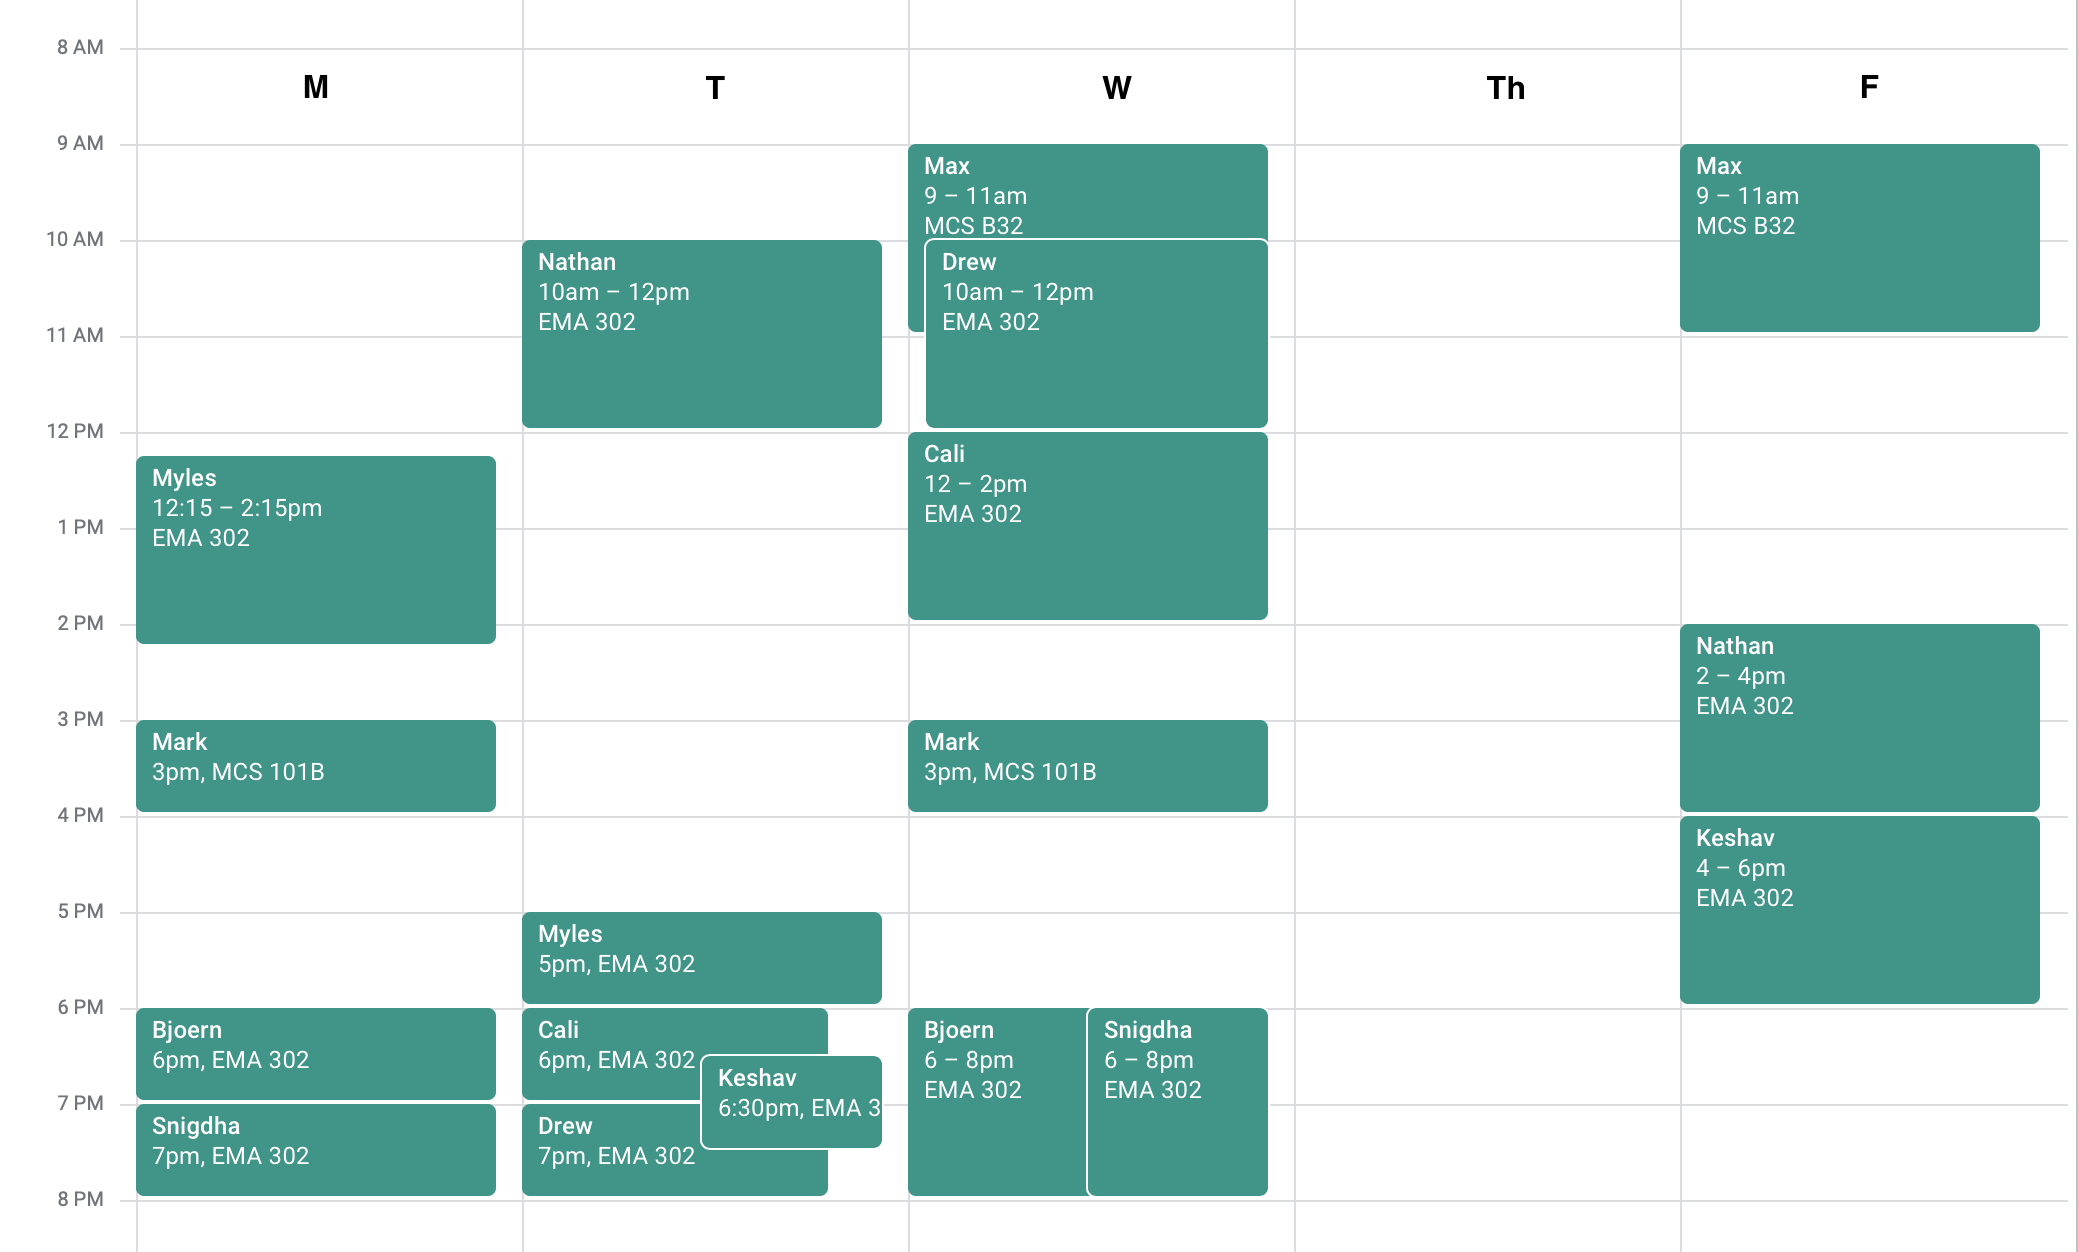
\includegraphics[width=\textwidth]{office-hours-schedule.png}}

\newpage

\section*{Academic Honesty}

You may discuss homework assignments with classmates, but you are 
solely responsible for what you turn in. Collaboration in the form of
discussion is allowed, but all forms of cheating (copying parts of a
classmate's assignment, plagiarism from books or old posted solutions)
are NOT allowed. We -- both teaching staff and students -- are expected
to abide by the guidelines and rules of the Academic Code of Conduct
(which is at
\url{http://www.bu.edu/dos/policies/student-responsibilities/}).

You can probably, if you try hard enough, find solutions for homework
problems online.    Given the nature of the Internet, this is
inevitable.   Let me make a couple of comments about that:
\begin{enumerate}
\item If you are looking online for an answer because you don't know how
  to start thinking about a problem, talk to a TF or myself, who may be
  able to give you pointers to get you started.  Piazza is great for
  this -- you can usually get an answer in an hour if not a few minutes.
\item If you are looking online for an answer because you want to see if
  your solution is correct, ask yourself if there is some way to verify
  the solution yourself.   Usually, there is.  You will understand what you have done
  \emph{much} better if you do that.
\item If you are looking online for an answer because you don't have
  enough time and are getting close to the assignment deadline, think about this:
  \begin{enumerate}
  \item what you are doing is intellectually dishonest,
  \item you are going to have to solve problems like this on the midterm
    and final, and
  \item you can miss up to two homeworks without penalty.
  \end{enumerate}
So ... it would be better to simply submit what you have at the deadline
(without going online to cheat) and plan to allocate more time for
homeworks in the future.
\end{enumerate}

\newpage
\section*{Course Schedule}

\textbf{IMPORTANT:} It is important to do the reading \emph{before} the class on

which it is based.   All readings are from LAA.
\\~\\
\small
\begin{centering}
\begin{tabular}{||l|p{3in}|l|l|l||}
\hline\hline
Date & Topics  & Reading & Assigned & Due  \\
\hline\hline
% Lay 1.1
1/21 & 1: Linear Equations & 1.1 & & \\
% Lay 1.2, 1.3
1/23& 1: Linear Equations (wrapup), 2: Numerics &  notes only &  H1 & \\
\hline

1/28 &  3: Row Reduction & 1.2 &  & \\
%  Lay 1.4, 1.5
1/30 & 4: Vector Equations  & 1.3 &  H2 & H1 \\
\hline

2/4 & 5: $A\mathbf{x} =\mathbf{b}$   & 1.4, 1.5, 1.6 &  & \\ % Include population movement example from 1.10 
2/6 & 6: Linear Independence  & 1.7 & H3 & H2 \\
\hline

%  Lay 1.7, 1.8, 1.9
2/11 & 7: Linear Transformations  (Guest Lecture) &  1.8 & & \\ 
% Lay 2.1
% note that this next lecture was too much material; spread into 2
% lectures next time
2/13 & 8: Matrices of Linear Transformations & 1.9 & H4 & H3 \\  
\hline

2/18 & \textbf{Substitute Monday; No Class} &&&\\
2/20 &9: Matrix Operations   & 2.1 &  H5 &  H4 \\ 
\hline

% Assigned Population Movement from 1.10 for homework - first
% state-transition problem (prep for Markov chains)
2/25 & 10: Matrix Inverse  & 2.2, 2.3 &  &  \\   
2/27 & 11: Markov Chains  &4.9 &  & H5 \\ % include the electrical circuit example 
\hline

% 
3/3 & 12: Matrix Factorizations  & 2.5 & &  \\ 
3/5 &  \textbf{Midterm} & &  H6 &  \\ 
  \hline

  3/10 & \textbf{Spring Break} &&& \\
  3/12 & \textbf{Spring Break} &&& \\
  \hline

% Lay 4.3
3/17 & 13: Computer Graphics  & 2.7 & & \\ 
3/19 & 14: Subspaces of $\mathbb{R}^n$  & 2.8 & H7 & H6\\ 
\hline

% Lay 4.4, 4.5
3/24 & 15: Dimension and Rank  & 2.9 &  & \\ 
3/26 & 16: Eigenvectors and Eigenvalues  &  5.1 & H8 & H7\\ 
\hline

% Lay 4.6, 5.1
3/31 & 17: The Characteristic Equation  & 5.2 & & \\ 
4/2 & 18: Diagonalization  & 5.3, 5.4 & H9 & H8\\  % Applications of eigen: markov, pagerank (exercises from 4.9)
\hline

% Lay 5.2, 5.3
4/7 & 19: PageRank  & notes only &  & \\
4/9 & 20: Inner Product, Length   & 6.1 & H10 & H9\\ 
\hline

% Lay 6.3, 6.5
4/14 &21: Orthogonal Sets & 6.2 &  & \\ 
  4/16 & 22: Least Squares   & 6.3, 6.5 & H11 & H10 \\
  \hline 


4/21 & 23: Linear Models  & 6.6 &  &\\ 
4/23 & 24: Symmetric Matrices  &7.1, 7.2, 7.3 & H12 & H11\\
\hline  
4/28 & 25: Singular Value Decomposition  & 7.4 &  &\\ 
4/30 & 26: Applications of SVD  && & H12 \\

\hline\hline

% to do next time:
% Lay 7.1, 7.2 

\end{tabular}\\
\end{centering}


\end{document}
